\pgfplotsset{compat=1.5}
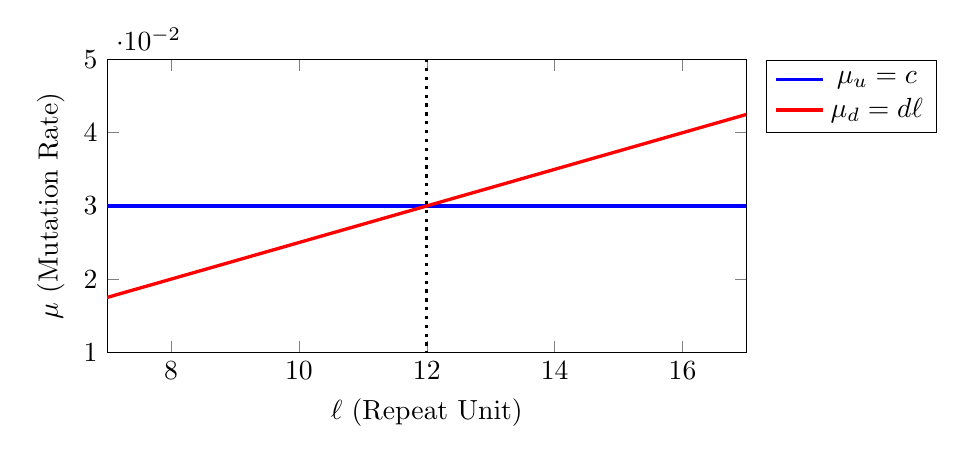
\begin{tikzpicture}
    \begin{axis}[
    width=0.8\linewidth, height=5.3cm,
    ylabel={$\mu$ (Mutation Rate)}, ymin=0.01, ymax=0.05,
    xlabel={$\ell$ (Repeat Unit)}, xmin=7, xmax=17,
    xtick={0, 2, 4, 6, 8, 10, 12, 14, 16, 18, 20, 22, 24, 26},
    samples=100, no markers, legend pos=outer north east, enlargelimits=false,
    domain=0:25
    ]
        \addplot+[very thick]{0.03};
        \addlegendentry{$\mu_u = c$};

        \addplot+[very thick]{0.0025*x};
        \addlegendentry{$\mu_d = d\ell$};

        \addplot+[very thick, black, dotted, forget plot] coordinates {(12, 0) (12, 0.05)};
    \end{axis}
\end{tikzpicture}